\documentclass[tikz,border=7pt]{standalone}
\usepackage{iftex}
\ifPDFTeX
  \PackageError{matrix-figure}{This figure requires XeTeX or Tectonic}{Compile with xelatex or tectonic.}
\fi
\usepackage{fontspec}
\usepackage{xeCJK}
\usepackage{amsmath}
\usepackage{unicode-math}
\usepackage{xcolor}
\usepackage{tikz}
\usetikzlibrary{arrows.meta,positioning}

\providecommand{\FigureUseLocalFonts}{0}
\ifnum\FigureUseLocalFonts=1
  \setmainfont{NotoSansCJKtc-Regular.otf}[Path=\FigureSansFontPath]
  \setsansfont{NotoSansCJKtc-Regular.otf}[Path=\FigureSansFontPath,BoldFont=NotoSansCJKtc-Bold.otf]
  \setCJKmainfont{NotoSansCJKtc-Regular.otf}[Path=\FigureSansFontPath]
  \setCJKsansfont{NotoSansCJKtc-Regular.otf}[Path=\FigureSansFontPath,BoldFont=NotoSansCJKtc-Bold.otf]
  \setmathfont{STIXTwoMath.otf}[Path=\FigureMathFontPath]
\else
  \setmainfont{Noto Sans CJK TC}
  \setsansfont{Noto Sans CJK TC}
  \setCJKmainfont{Noto Sans CJK TC}
  \setCJKsansfont{Noto Sans CJK TC}
  \setmathfont{STIX Two Math}
\fi

\definecolor{FigureInk}{HTML}{253142}
\definecolor{PanelFill}{gray}{0.96}
\definecolor{RowShade}{gray}{0.86}
\definecolor{ColumnShade}{gray}{0.74}
\definecolor{ResultShade}{gray}{0.58}
\definecolor{FocusShade}{gray}{0.68}
\definecolor{GuideShade}{gray}{0.80}

\newcommand{\MatrixCell}[2]{%
  \tikz[baseline=(value.base)]{\node[fill=#1,rounded corners=0.4pt,inner sep=2.2pt,
    minimum width=1.35em,minimum height=1.35em] (value) {$#2$};}%
}
\newcommand{\RowCell}[1]{\MatrixCell{RowShade}{#1}}
\newcommand{\ColumnCell}[1]{\MatrixCell{ColumnShade}{#1}}
\newcommand{\ResultCell}[1]{\MatrixCell{ResultShade}{#1}}
\newcommand{\FocusCell}[1]{\MatrixCell{FocusShade}{#1}}

\tikzset{
  figure/.style={font=\sffamily,text=FigureInk,>={Stealth[length=3.5mm,width=2.5mm]}},
  panel/.style={draw=FigureInk,line width=0.9pt,rounded corners=1.5mm,fill=PanelFill,align=center},
  flow/.style={-{Stealth},line width=1.05pt,draw=FigureInk},
}


\begin{document}
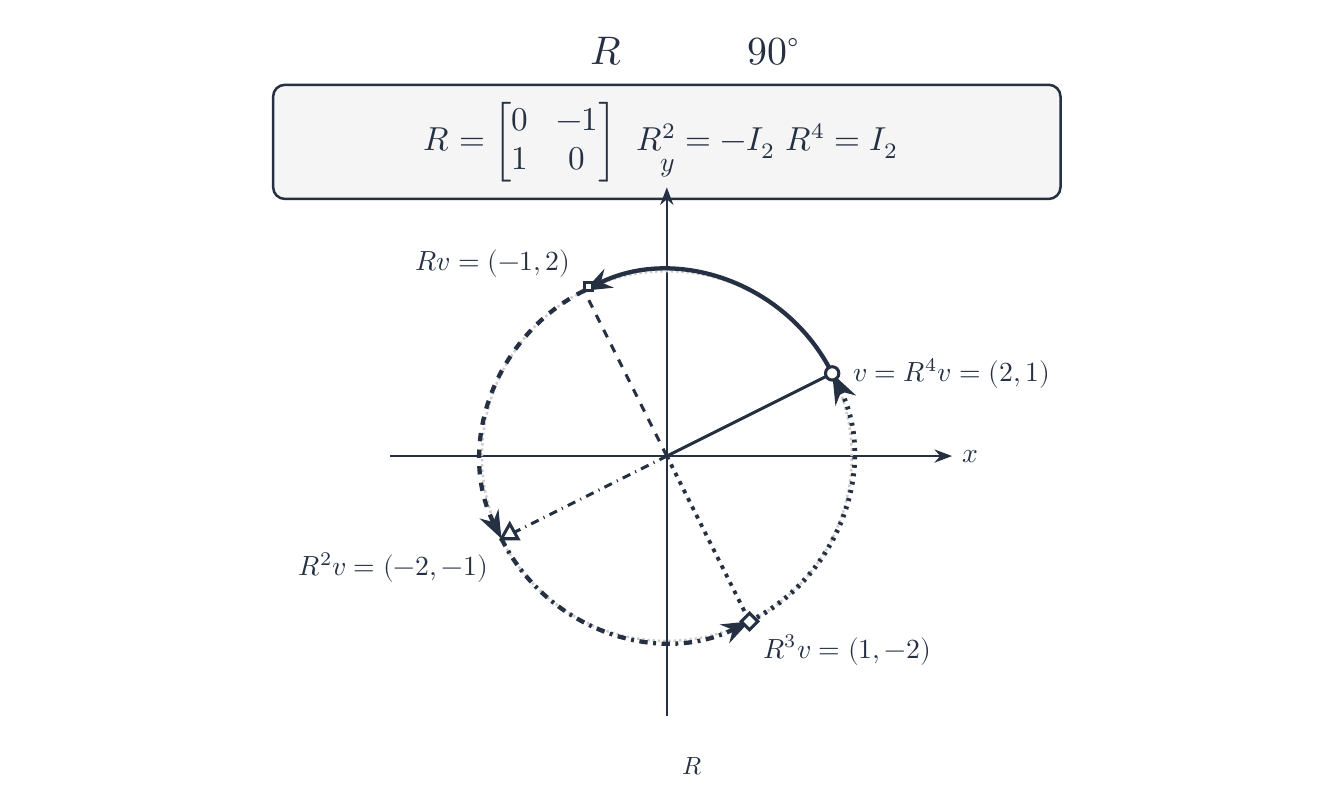
\begin{tikzpicture}[figure,scale=1.05]
  \node[font=\bfseries\Large,align=center,text width=16cm] at (7.5,8.65)
    {每次左乘 $R$ 都使向量逆時針旋轉 $90^\circ$};
  \node[panel,minimum width=10.0cm,minimum height=1.45cm] at (7.5,7.55) {%
    \large$R=\begin{bmatrix}0&-1\\1&0\end{bmatrix}$，
    $R^2=-I_2$，$R^4=I_2$
  };

  \begin{scope}[shift={(7.5,3.75)}]
    \draw[-{Stealth},FigureInk,line width=0.75pt] (-3.35,0) -- (3.45,0) node[right] {$x$};
    \draw[-{Stealth},FigureInk,line width=0.75pt] (0,-3.15) -- (0,3.25) node[above] {$y$};
    \draw[GuideShade,densely dotted,line width=0.9pt] (0,0) circle[radius=2.236];

    \draw[FigureInk,line width=1.1pt] (0,0) -- (2,1);
    \draw[FigureInk,dashed,line width=1.1pt] (0,0) -- (-1,2);
    \draw[FigureInk,dash dot,line width=1.1pt] (0,0) -- (-2,-1);
    \draw[FigureInk,dotted,line width=1.4pt] (0,0) -- (1,-2);

    \draw[flow,line width=1.55pt] (2,1)
      arc[start angle=26.565,end angle=116.565,radius=2.236];
    \draw[flow,dashed,line width=1.55pt] (-1,2)
      arc[start angle=116.565,end angle=206.565,radius=2.236];
    \draw[flow,dash dot,line width=1.55pt] (-2,-1)
      arc[start angle=206.565,end angle=296.565,radius=2.236];
    \draw[flow,dotted,line width=1.75pt] (1,-2)
      arc[start angle=296.565,end angle=386.565,radius=2.236];

    \filldraw[fill=white,draw=FigureInk,line width=1.1pt] (2,1) circle[radius=2.3pt];
    \filldraw[fill=white,draw=FigureInk,line width=1.1pt] (-1,2) rectangle ++(0.10,0.10);
    \filldraw[fill=white,draw=FigureInk,line width=1.1pt] (-2,-1) -- ++(0.10,0.18) -- ++(0.10,-0.18) -- cycle;
    \filldraw[fill=white,draw=FigureInk,line width=1.1pt] (1,-2) ++(0,0.10) -- ++(0.10,-0.10) -- ++(-0.10,-0.10) -- ++(-0.10,0.10) -- cycle;

    \node[right=4pt] at (2,1) {$v=R^4v=(2,1)$};
    \node[above left=2pt] at (-1,2) {$Rv=(-1,2)$};
    \node[below left=2pt] at (-2,-1) {$R^2v=(-2,-1)$};
    \node[below right=2pt] at (1,-2) {$R^3v=(1,-2)$};
  \end{scope}

  \node[font=\small] at (7.5,0.0)
    {四個四分之一圓弧各代表再左乘一次 $R$；第四次回到原向量。};
\end{tikzpicture}
\end{document}
